%
% File naaclhlt2016.tex
%

\documentclass[11pt,letterpaper]{article}
\usepackage{naaclhlt2016}
\usepackage{times}
\usepackage{latexsym}
\usepackage{amsmath, amssymb, amsthm}
\usepackage{multirow}
\usepackage[hidelinks]{hyperref}
\usepackage{hyperref}
\usepackage{float}
\hypersetup{
    bookmarks=false,         % show bookmarks bar?
    unicode=false,          % non-Latin characters in Acrobat’s bookmarks
    colorlinks=true,       % false: boxed links; true: colored links
    linkcolor=red,          % color of internal links (change box color with linkbordercolor)
    citecolor=black,        % color of links to bibliography
    filecolor=magenta,      % color of file links
    urlcolor=blue           % color of external links
}
\usepackage{tikz}
\usetikzlibrary{arrows,shapes,snakes,automata,backgrounds,petri,positioning}


%\naaclfinalcopy % Uncomment this line for the final submission
\def\naaclpaperid{***} %  Enter the naacl Paper ID here

% To expand the titlebox for more authors, uncomment
% below and set accordingly.
% \addtolength\titlebox{.5in}    

\newcommand{\fix}{\marginpar{FIX}}
\newcommand{\new}{\marginpar{NEW}}
\newcommand{\NIL}{\mbox{\textsc{nil}}}
\newcommand{\qtext}[1]{\texttt{#1}}

\title{Coherence model for entity resolution (name?)}

% Author information can be set in various styles:
% For several authors from the same institution:
% \author{Author 1 \and ... \and Author n \\
%         Address line \\ ... \\ Address line}
% if the names do not fit well on one line use
%         Author 1 \\ {\bf Author 2} \\ ... \\ {\bf Author n} \\
% For authors from different institutions:
% \author{Author 1 \\ Address line \\  ... \\ Address line
%         \And  ... \And
%         Author n \\ Address line \\ ... \\ Address line}
% To start a seperate ``row'' of authors use \AND, as in
% \author{Author 1 \\ Address line \\  ... \\ Address line
%         \AND
%         Author 2 \\ Address line \\ ... \\ Address line \And
%         Author 3 \\ Address line \\ ... \\ Address line}
% If the title and author information does not fit in the area allocated,
% place \setlength\titlebox{<new height>} right after
% at the top, where <new height> can be something larger than 2.25in
\author{Author1 \and Author2\\
	    Google Inc. \\
	    1600 Amphitheatre Pkwy\\
	    Mytown, NY 10000, USA\\
	    {\tt author1@google.com}}

\date{}

\begin{document}

\maketitle

\begin{abstract}
Entity resolution is the task of linking each mention of an entity in text to the corresponding record in a knowledge base (KB). Coherence models for entity resolution encourage all referring expressions in a document to resolve to entities that are related in the KB. 
Such models are often specified via a graph whose vertices correspond to candidate entities, and weighted edges to entity relations. We present a new graph-based coherence method which attempts to find the best link for each candidate and relies on the max-sum algorithm for inference.  Applying our approach to the output of an existing system improves its performance on three (out of three) benchmarks, yielding state-of-the-art results on the TAC KBP 2011 and 2012 tasks.
\end{abstract}


\section{Introduction}
%
Entity resolution is the task of mapping each mention of an entity in a document to the corresponding record in a knowledge base (KB) \cite{BunescuP06,Cucerzan07,Dredze2010,Hachey2013130}.  
 %with numerous applications \cite{Gabrilovich2007,Lin2012,Kwiatkowski2011,finin2009Coreference,mayfield2009cross}. 
%Key applications 
%are to information extraction  and grounded semantic parsing. %text classification~\cite{Gabrilovich2007}, 
%information extraction~\cite{Lin2012} and grounded semantic parsing~\cite{Kwiatkowski2011}. 
%It can also provide a valuable signal to other language-processing tasks, including part-of-speech tagging, parsing, and coreference resolution~\cite{finin2009Coreference,mayfield2009cross}.
%Entity resolution
This is a challenging problem, as referring expressions are often ambiguous on their own, and can only be resolved given appropriate context. For example, the mention \qtext{Beirut} may refer to the capital of Lebanon, to the indie band from New Mexico, or to a drinking game. Names may also refer to entities that are not in the KB, a problem known as \emph{{\NIL} detection}. 
Entity resolution applications include numerous language-processing tasks  \cite{Gabrilovich2007,Lin2012,finin2009Coreference,mayfield2009cross}. %Kwiatkowski2011

Systems for entity resolution typically consist of a \emph{mention model}, a \emph{context model}, and a \emph{coherence model}. The mention model establishes a link between each entity and its textual representations, also called aliases or surface forms. The context model helps resolve an ambiguous phrase using textual features extracted from the surrounding context, such as the enclosing sentence and salient noun phrases in the document. The coherence model encourages all mentions to resolve to entities that are related to each other in the KB. 

Coherence models are often specified via a graph whose vertices are candidate entities for all mentions, and whose edges indicate known relations\footnote{An exception to this framework are topic models in which a topic may generate both entities and words, e.g. \cite{HanS12,houlsby2014scalable}.}. Vertex weights correspond to prior scores for candidate entities, while edge weights correspond to some notion of relation strength. There exist different ways to leverage such a graph for disambiguation purposes. Some systems compute an overall ``relatedness'' score for each candidate as the average of adjacent edge weights \cite{Milne2008,Ferragina10}. \newcite{Ratinov11} use relation scores as features in a ranking support vector machine. \newcite{KulkarniSRC09} formulate the task as an integer linear program and find solutions via a convex relaxation, while \newcite{Hoffart2011} extract a dense subgraph from the original graph. More recent systems \cite{Han2011,He13,Alhelbawy14,Pershina2015} use variants of the PageRank algorithm \cite{PageRank} to re-score candidates.  

In this work, we formulate inference as finding the highest-weight subgraph in which each candidate has a directed edge to \emph{at most} one other candidate. This can roughly be seen as maximizing over neighboring edge weights as opposed to averaging; however, it is slightly more computationally involved since an edge between two entities is allowed only if the corresponding mentions resolve to them. We specify the objective and constraints using binary edge-indicator variables, and find the maximum-a-posteriori solution using the max-sum algorithm \cite{Kschischang2001}. TODO: more motivation / rationale.
 
We use our technique to re-score candidates generated by Plato \cite{Lazic2015}, a recent entity resolution system that has highly competitive performance and does not include a coherence component. This leads to performance improvements on three benchmarks, and yields new state-of-the-art results on the TAC KBP 2011 and 2012 datasets.


\begin{figure*}[!ht]
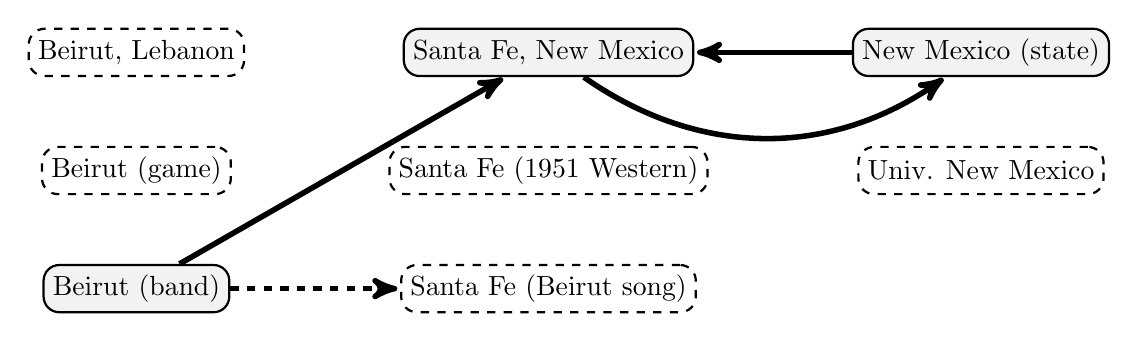
\begin{tikzpicture}[node distance=1.5cm,>=stealth',bend angle=35,auto]
  \tikzstyle{candidate}=[rectangle,dashed,rounded corners=2mm,thick,draw=black,fill=white,minimum size=6mm]
  \tikzstyle{selected} = [rectangle,rounded corners=2mm,thick,draw=black,fill=gray!10,minimum size=6mm]
  \tikzstyle{mention}=[rectangle,thick,draw=black!75,
  			  fill=black!10,minimum size=6mm]
  \tikzstyle{every label}=[black]

 \begin{scope}
    % First mention.
   % \node [mention] (m1){\qtext{Beirut}};
   % \node [candidate] (c11) [label=above:0.5] {Beirut, Lebanon};
   \node [candidate] (c11) {Beirut, Lebanon};
    \node [candidate] (c12) [below of=c11]  {Beirut (game)};
        \node [selected] (c13)  [below of=c12] {Beirut (band)};

   % Second mention.
   % \node [mention] [right=3cm of m1](m2){\qtext{Santa Fe}};
    \node [selected] (c21) [right=2cm of c11] {Santa Fe, New Mexico};
        \node [candidate] (c22) [below of=c21]  {Santa Fe (1951 Western)};
    \node [candidate] (c23)  [below of=c22] {Santa Fe (Beirut song)};

      
     % Third mention.
   % \node [mention] [right=3cm of m2](m3){\qtext{New Mexico}};
    \node [selected] (c31) [right=2cm of c21] {New Mexico (state)};
    \node [candidate] (c32)  [below of=c31] {Univ. New Mexico};
 
      
   %\path (c13) edge [post,line width=2pt] node[above]{0.5} (c21);
   \path (c13) edge [post,line width=2pt] (c21);
   \path (c13) edge [post,dashed,line width=2pt] (c23);
   \path (c31) edge [post,line width=2pt] (c21);
   \path (c21) edge [post,line width=2pt,bend right] (c31);
  \end{scope}
\end{tikzpicture}
\caption{Example coherency graph for mentions $\qtext{Beirut}$, $\qtext{Santa Fe}$ and $\qtext{New Mexico}$. Solid lines indicate a valid solution subgraph, where each selected candidate has at most one outgoing edge to another candidate. TODO: better example?}
\label{fig:graph}
\end{figure*}


\section{Model}

Similarly to prior work, we specify the model using a graph in which vertices are candidate entities for each mention in the document, and directed edges are known relations between entities. Each vertex $(m, c)$, corresponding to candidate $c$ for mention $m$, is associated with a prior score $t_{mc}$ for $m$ resolving to $c$.  Similarly, each edge from $(m,c)$ to $(m',c')$ is associated with a score $s_{cc'}$, indicating the strength of the relation between the  two candidate entities. 
Edges are directed because pairwise relations are often asymmetric, especially if one entity is more common than the other (for example, Springfield NE and Nebraska). We do not allow edges between candidates for the same mention. 

Our goal is to find the highest-weight subgraph such that (1) we select exactly one candidate for each mention, and (2) each candidate has at most one \emph{outgoing} edge to another candidate. We place no constraints on the number of incoming edges; however, note that edges can only exist between selected candidates. See Figure \ref{fig:graph} for an example. TODO: some rationale (max wt, salient entities).

For notational convenience, we augment the graph with a special vertex $(0, 0)$ that all other vertices link to with edge weight $0$ and require each candidate to have exactly one outgoing edge. An edge from $(m, c)$ to $(0, 0)$ then indicates that $m$ resolves to $c$ and $c$ has no relations to other resolved entities. 

Let $x_{mc}^{m'c'}$ be a binary variable indicating whether a directed edge from $(m, c)$ to $(m', c')$ is present in the solution subgraph or not. We will use ``:'' to indicate the entire range of an index, so that $x_{mc}^{::}$ is the set of variables corresponding to all outgoing edges from $(m,c)$.  According to our formulation, mention $m$ will resolve to candidate $c$ if vertex $(m,c)$ has an outgoing edge, or $ \max x_{mc}^{::}=1$. We now specify the overall objective and constraints using these binary edge variables. Maximize:
\begin{align}
E(x_{::}^{::}) =& \sum_{(m, c), (m',c')} t_{mc} \;x^{m'c'}_{mc}  + \sum_m \phi_m( x_{m:}^{::}) \nonumber \\
&+ \sum_{(m,c), (m', c') \in \mathcal{E}} \sigma_{mc}^{m'c'}(x_{mc}^{m'c'}, x_{m'c'}^{::}) \\ \nonumber \\
\phi_{m}&= 
\begin{cases} 
0 & \text{if} \; \sum_{c, (m',c')} x^{m'c'}_{mc} = 1 \\
-\infty & \text{otherwise.}
\end{cases} \\ \nonumber \\
\sigma_{mc}^{m'c'} &= %(x_{mc}^{m'c'}, x_{m'c'}^{::}) &=
\begin{cases}
 s_{cc'} & \text{if $x_{mc}^{m'c'}=1$ and $\max x_{m'c'}^{::} =1$} \\
 -\infty & \text{if $x_{mc}^{m'c'}=1$ and $\max x_{m'c'}^{::}=0$} \\
  0 & \text{ if $x_{mc}^{m'c'} = 0$ } 
 \end{cases}
\end{align}
Here, the factors $t_{mc} x_{mc}^{m'c'}$ incorporate the prior score that mention $m$ resolves to candidate entity $c$. 
Factors $\phi_m$ enforce the constraints that each mention resolves to exactly one candidate and has exactly one outgoing edge. 
Finally, factors $\sigma_{mc}^{m'c'}$ add the score $s_{cc'}$ if the edge corresponding to $x_{mc}^{m'c'}$ is included in the solution subgraph. They also enforce the constraint that $x_{mc}^{m'c'}$ cannot be included in the solution unless the vertex $(m', c')$ is included as well, that is  $\max x_{m'c'}^{::} = 1$.

%


\section{Inference}

\subsection{Max-sum algorithm}
The max-sum algorithm is an iterative algorithm for maximum-a-posteriori (MAP) inference:
\begin{equation}
{\bf x}^{MAP} = \arg \max_{\bf x} p({\bf x}) = \arg \max_{\bf x} \sum_a \phi_a({\bf x}_a).
\end{equation}
 It can be described in terms of messages $\mu_{\phi \rightarrow X}(x)$ sent from factors $\phi$ to their neighboring variables. At convergence, each variable is assigned to the value that maximizes its \emph{belief} $b(x)$, defined as the sum of all incoming messages. The message updates have the following form:
\begin{align}
\mu_{\phi_a \rightarrow X_i}(x_i) =& \max_{ {\bf x}_a \setminus x_i } \bigg[ \phi_a({\bf x}_a) + \sum_{j \neq i} q_j^{\setminus a}(x_j)\bigg]
\label{eq:damping}
\end{align}
\noindent where $q_j^{\setminus a}$ is the sum of all messages except the one from factor $\phi_a$. For binary variables, it is often convenient to update log-odds messages and beliefs, $\mu_{\phi \rightarrow X} \equiv \mu_{\phi \rightarrow X}(1)-\mu_{\phi \rightarrow X}(0)$. It is also often beneficial to use damped message updates
\begin{align}
\mu^{t+1} &= \alpha \mu^t + (1 - \alpha) \mu^{update}, \;\;\; \alpha \in [0, 1)  
\end{align}
where $t$ is the iteration and $\mu^{update}$ is the message defined in Eq. \ref{eq:update}.

\section{Max-sum in the coherence model}

Our coherence model has three types of factors, corresponding to the prior scores, relation scores, and constraints. The messages for prior factors $t_{mc} x_{mc}^{m'c'}$ do not change across iterations and are simply equal to $t_{mc}$. The message from factor $\phi_m$ to a variable $x_{mc}^{m'c'}$ has the form
\begin{align}
\mu_{\phi_m \rightarrow x_{mc}^{m'c'}} = -\max \{ q_{m:}^{::} \; \setminus \; q_{mc}^{m'c'}\} 
\end{align}
where each $q_{mi}^{jk}$ is the sum of all messages to $x_{mi}^{jk}$ except that from $\phi_m$. In effect, the message lowers the belief for $x_{mc}^{m'c'}$ by the highest $q$ of a competing edge.

The message from factor $\sigma_{mc}^{m'c'}$ to the corresponding edge variable $x_{mc}^{m'c'}$  is:
\begin{align}
\mu_{\sigma_{mc}^{m'c'} \rightarrow x_{mc}^{m'c'}} &= s_{cc'} + \min(0, \max_{(i, j)} \tilde{q}_{m'c'}^{ij} )
\end{align}
where $\tilde{q}$ is the sum of all messages except from $\sigma$. In this case, the message corresponds to the edge weight $s_{cc'}$, and gets discounted if all of the $\tilde{q}$s for candidate $(m', c')$ are negative. Finally, the message from $\sigma_{mc}^{m'c'}$ to a variable $x_{m'c'}^{ij}$ is
\begin{align}
\mu_{\sigma_{mc}^{m'c'} \rightarrow x_{mc}^{ij}} &= \max(0, s_{cc'} + \tilde{q}_{mc}^{m'c'}) \\ 
 &- \max (0, s_{cc'} + \tilde{q}_{mc}^{m'c'} + \max_{(k,l) \neq (i, j)} \tilde{q}_{m'c'}^{kl}  ) \nonumber
\end{align}

We initialize to zero all messages except those from prior factors, and use updates with damping $\alpha=0.9$ .  We iteratively update relation factors $\sigma$ and corresponding constraint factors $\phi$ for five cycles over all factors. Following the updates, each mention $m$ is assigned the candidate with the highest belief for any edge: $c^* = {\arg \max}_{c} (\max b_{mc}^{::})$.


\begin{table*}[ht]
\small
\centering
\begin{tabular}{|l|l|l|c|c|c|}
\hline 
\bf Data & \bf Plato & \bf Model & \bf In-KB & \bf Overall & ${\bf B^{3+}F_1}$ \\ 
& \bf cand. recall &  & \bf accuracy & \bf accuracy & \\ \hline
TAC 2011 & 84.8 & \newcite{Cucerzan2011} &- & 86.8 &  {84.1} \\
&& Plato \cite{Lazic2015} & 79.3 & 86.5 & 84.0 \\
&& Plato with coherence & {\bf 81.2} & {\bf 87.0} & {\bf 84.5} \\
\hline
\hline
TAC 2012 & 83.2 &\newcite{Cucerzan2012}  Run 1 & 72.0 & 76.2 & 72.1  \\
& &\newcite{Cucerzan2012} Run 3 & 71.2 & {76.6} & {\bf 73.0} \\
& &Plato \cite{Lazic2015} & {74.2} & {76.6} & 71.2 \\
& &Plato with coherence & {\bf 75.1} & {\bf 77.3} & {72.2} \\
\hline
\end{tabular}
\caption{ \label{table:tac_results} TAC KBP evaluation results for our model and previous highest-accuracy systems.  }
\end{table*}

\begin{table*}[ht]
\small
\centering
\begin{tabular}{|l|l|l|c|}
\hline 
\bf Data & \bf Plato & \bf Model & \bf In-KB  \\ 
& \bf cand. recall &  & \bf accuracy \\ \hline
CoNLL all & 91.7 & \newcite{Pershina2015} & {\bf 91.8}  \\
&& Plato \cite{Lazic2015} & 86.5 \\
&& Plato with coherence & 86.9  \\
\hline
\hline
CoNLL test-b &  & \newcite{Chisholm2015} & {\bf 88.7} \\
& &Plato \cite{Lazic2015} & {86.4}  \\
& &Plato with coherence & {87.1} \\
\hline
\end{tabular}
\caption{ \label{table:conll_results} CoNLL evaluation results for our model and previous highest-accuracy systems. }
\end{table*}

\section{Experimental evaluation}

We use the output of Plato \cite{Lazic2015} as our baseline, as well as to generate candidates and initial scores $t_{mc}$. Plato does not have an explicit coherence model; however, it does capture some coherence information as referrent phrases are included as string features. Plato outputs posterior probabilities of candidates for each mention $p(c|m)$. Our model has no probabilistic interpretation, and we simply set $t_{mc} = \ln p(c|m) - \ln (1 - p(c|m))$, so that likely candidates get positive scores. We set edge weights to $s_{cc'} = \ln n_{cc'} + \beta$, where $n_{cc'}$ is the number of outlinks from the Wikipedia page of $c$ to the page of $c'$ and $\beta=0.7$. We consider up to $k=3$ candidates for each mention; if the Plato posterior for the top candidate exceeds $0.9$, we only include the top candidate in the graph.

We evaluate our approach on the same three corpora as \newcite{Lazic2015}. The CoNLL dataset ~\cite{Hachey2013130} contains 1,393 articles with about 34K
mentions, and the standard performance metric is mention-averaged accuracy.
The TAC KBP datasets \cite{TAC2011,TAC2012} include 2,226 mentions (2012) and 2,250 mentions (2011), of which roughly half are linkable to the reference KB. The competition evaluation includes $\NIL$ entities;
participants are required to cluster $\NIL$ mentions across documents
so that all mentions of each unknown entity are assigned a unique
identifier. We use the same $\NIL$ cluster labels as Plato. For these datasets, we report in-KB accuracy, overall accuracy (including $\NIL$ mentions), and the competition metric $B^{3+} F_1$. 

We show the performance of the Plato baseline, Plato with coherence, and the best results reported in literature in Tables \ref{table:tac_results} and \ref{table:conll_results}.  The coherence model improves performance on all three datasets, yielding new state-of-the-art results on the TAC KBP datasets. While coherence also leads to improved performance on CoNLL, the overall system does not surpass the state of the art. One reason for this is that the candidate recall of the baseline system (an upper bound on accuracy) is relatively low -- below the accuracy of the system of \cite{Pershina2015}. 

\section{Discussion and conclusion}

We have described a simple new graph-based approach to coherence, where each candidate can have at most one relation to another candidate in the solution subgraph. Our approach in effect maximizes over relation scores rather than averaging, which ensures that the scores are not diluted. Compared to the recently popular PageRank methods, our model can only exploit one-hop links. TODO why this is good and multihop relations spurious.

%\section*{Acknowledgments}

%Do not number the acknowledgment section.

\bibliography{refs}
\bibliographystyle{naaclhlt2016}


\end{document}
